\documentclass[../root]{subfiles}
\graphicspath{{_images/}{../_images/}}

\begin{document}

    \chapter{Racial Bias in Bail Decisions}

    \begin{shortsummary}
        \begin{itemize}
            \item \authoryear{ArnoldEtal}
            \item \RQ{Is racial bias exist in the context of bail decisions? If so, is the bias are driven by racial anumus, or inaccurate racial stereotypes, or any other form of bias?}
            \item \answer{IVs and MTEs, using a measure of bail judges' leniency as an instrument.}
            \item \result{Bail judges are racially biased against black defendants. The bias is driven by bail judges relying on inaccurate stereotypes.}
        \end{itemize}
    \end{shortsummary}

    \section{Introduction}
    \paragraph{Racial disparities in U.S. criminal justice system}

    \begin{itemize}
      \item Compared to observably similar whites, blacks are
      \begin{itemize}
        \item are more likely to be searched for contraband (Antonovics and Knight 2009)
        \item more likely to experience police force (Fryer 2016)
        \item more likely to be charged with a serious offense (Rehavi and Starr 2014)

        \ldots
      \end{itemize}
    \end{itemize}

    \paragraph{Possible mechanisms to explain the discrimination}

    \begin{enumerate}
      \item statistical discrimination
      \begin{itemize}
        \item the use of observable group traits (such as race) to form accurate beliefs about the unobservable characteristics of defendants (e.g., Phelps 1972; Arrow 1973).
      \end{itemize}
      \item various forms of racial bias
      \begin{itemize}
        \item racial animus (e.g., Becker 1957)
        \item inaccurate racial stereotypes (e.g., Bordalo et al. 2016).
      \end{itemize}
    \end{enumerate}

    \paragraph{Becker (1957, 1993)'s "outcome test"}

    \begin{itemize}
      \item Distinguishing between these contrasting explanations remains an empirical challenge.
      \item Becker's test
      \begin{itemize}
        \item compares the success or failure of decisions across groups at the margin.
        \item the outcome will be identical for marginal white and marginal black defendants if bail judges are racially unbiased
      \end{itemize}
    \end{itemize}

    \paragraph{the Inframarginality problem}

    \begin{itemize}
      \item Comparisons are biased when whites and blacks have different risk distributions.
      \item Two papers dealing with the problem:

      Knowles, Persico, and Todd (2001), and Anwar and Fang (2006)

      \item However, they have been critiqued for its reliance on restrictive assumptions about the unobserved risk of blacks and whites (e.g., Brock et al. 2012).
    \end{itemize}

    \paragraph{Bail decisions}

    \begin{itemize}
      \item Racial disparities are particularly prominent in the setting of bail.
      \begin{itemize}
        \item in the data of this paper, black defendants are 3.6 percentage points more likely to be assigned monetary bail than white defendants
        \item conditional on being assigned monetary bail, receive bail amounts that are \$9,923 greater
      \end{itemize}
      \item If the bail judges are racially biased against blacks, marginal white defendants will have higher rates of pretrial misconduct than marginal black defendants.
    \end{itemize}

    Bail is an ideal setting to test for racial bias for a number of reasons.

    \begin{itemize}
      \item The legal  objective of bail judges is narrow, straightforward, and measurable: allow most defendants to be released while minimizing the risk of pretrial misconduct.
      \item Mostly untrained bail judges must make on-the-spot judgments with limited information and little to no interaction with defendants.
      \item Bail decisions are extremely consequential for both white and black defendants.
      \begin{itemize}
        \item Detained defendants suffer about \$30,000 in lost earnings and government benefits alone (Dobbie, Goldin, and Yang 2018).
      \end{itemize}
    \end{itemize}

    \paragraph{Empirical Approach}

    \begin{itemize}
      \item Quasi-random assignment of bail judges to identify theh differences in pretrial misconduct rates.
      \begin{enumerate}
        \item the standard instrumental variables (IVs)
        \begin{itemize}
          \item LATEs for white and black defendants near the margin of release.
          \item is adequate for the Becker's test that explore the local treatment effect.
        \end{itemize}
        \item the marginal treatment effects (MTEs)
        \begin{itemize}
          \item estimate judge-specific treatment effects for white and black defendants at the margin of release.
        \end{itemize}
      \end{enumerate}
    \end{itemize}

    \paragraph{Summary of the Results}

    \begin{itemize}
      \item Data: administrative court data from Miami and Philadelphia.
      \item Significant racial bias against black defendants.
      \begin{itemize}
        \item marginally released white defendants are 22.2(IV) to 23.1(MTE) percentage points more likely to be rearrested prior to disposition.
        \item Naive OLS estimates indicate racial bias against white defendants.
      \end{itemize}
      \item the form of racial bias: inaccurate stereotypes
      \begin{itemize}
        \item both white and black bail judges exhibit racial bias against black defendants.
      \end{itemize}
    \end{itemize}

    \section{An Empirical Test of Racial Bias}

    Theoretical framework that follows the previous literature.

    \subsection{Overview of the Bail Systems}

    \begin{itemize}
      \item In the United States, bail judges decide whether to detain or release a defendant at the bail hearing.
      \begin{itemize}
        \item The hearing last only a few minutes
        \item They have a number of potential options for releasing defendants.
        \item There are substantial diffenrences across judges.
      \end{itemize}
      \item They are meant to balance two competing objectives.
      \begin{enumerate}
        \item To avoid undue punishment before the defendant have not been convicted.
        \item To minimize the risk of pretrial misconduct.
      \end{enumerate}
      \item One important difference: experience of the bail judges.
      \begin{itemize}
        \item Philadelphia: judges are full-time specialists.
        \item Miami: judges are part-time.
      \end{itemize}
    \end{itemize}

    \subsection{Model of Judge Behavior}

    \begin{itemize}
      \item The expected probability of pretrial misconduct is
      \[
      E[\alpha_i | \mathbf{V}, r_i]
      \]
      where
      \begin{itemize}
        \item $i, j$: denotes the defendant and the bail judge, respectively.
        \item $r_i \in \{\text{W}, \text{B}\}$: race
        \item $\mathbf{V}$: All case and defendant characteristics.
      \end{itemize}

      \item Let $t_r^j$ be the benefit of release for defendant of race $r$, then for the marginal defendant, the following equation holds.
      \[
      E[\alpha_i | \mathbf{V}, r_i] = \alpha_r^j = t_r^j(\mathbf{V})
      \]
      \item Possible sources of racial discrimination.
      \begin{enumerate}
        \item Taste-Based Discrimination
        \item Racial Biased Prediction Errots in Risk
        \item Statistical discrimination
      \end{enumerate}

      \item[1, 2] If judge $j$ is biased, then $\alpha_W^j > \alpha_B^j$; the marginal white defendants have higher probability of misconduct than the black ones.
      \item[3] The probability of misconduct is the same between the marginal black/white defendant.
    \end{itemize}

    \subsection{Empirical Test of Racial Bias in Bail Setting}

    \begin{itemize}
      \item Outcome: rate of pretrial misconduct; treatment: release
      \item Definition of the average level of racial bias amoung bail judges:
      \begin{align*}
        D^{*, w} &= \sum_{j = 1}^J w^j \left( t_W^j - t_B^j \right) \\
        &= \alpha_W^{*, w} - \alpha_B^{*, w}
      \end{align*}
      for some weighting scheme across all bail judges $j = 1, \ldots, J$.
      \begin{itemize}
        \item weighting scheme $w^j$ is determined by the treatment effect of interest.
      \end{itemize}
      \item Standard OLS will not recover unbiased estimates of racial bias.
      \begin{itemize}
        \item Omitted variable (unobservable for the econometricians) bias
        \item Lack of the assumption: either identical risk distribution or constant treatment effects between the races.
      \end{itemize}
      \item Two complementary estimators are to be developed: IV and MTE
    \end{itemize}

    \paragraph{Setup} cf. Imbens and Angrist (1994)

    \begin{itemize}
      \item Assigned judge's propensity for pretrial release for defendant-case $i$: $Z_i$
      \item Assumptions for $Z_i$ to be valid as an instrumental variable
      \begin{enumerate}
        \item Existance: $\textit{Cov}(\text{Released}_i, Z_i) \neq 0$,
        \item Exclusion: $\textit{Cov}(Z_i, \mathbf{v}_i) = 0$ where $\mathbf{v}_i = \mathbf{U}_i + \epsilon_i$.
        \item Monotonicity: $\text{Released}_i (z_j) - \text{Released}_i (z_{j - 1})$
      \end{enumerate}
    \end{itemize}

    \paragraph{the standard IV}

    \begin{itemize}
      \item the standard IV-weighted level of racial bias:
      \begin{align*}
        D^{*, \text{IV}} &= \sum_{j = 1}^J \lambda^j \left( t_W^j - t_B^j \right)
      \end{align*}
      \item Using the treatment effects of compliers $\alpha_r^{j, j - 1} \in (t_r^{j - 1}, t_r^j]$, the IV estimator that uses judge leniency as an instrument:
      \begin{align*}
        D^{\text{IV}} &= \sum_{j = 1}^J \lambda^j_W \alpha_W^{j, j - 1} - \sum_{j = 1}^J \lambda^j_B \alpha_B^{j, j - 1}
      \end{align*}
      \item If (i) $Z_i$ is continuous and $\lambda_r^j$ is constant by race, $D^{\text{IV}}$ provides the consistent estimate of $D^{*, \text{IV}}$.
    \end{itemize}


    \paragraph{the MTE}

    \begin{itemize}
      \item the true equal-weighted MTE
      \begin{align*}
        D^{*, \text{MTE}} &= \sum_{j = 1}^J \dfrac{1}{J} \left( t_W^j - t_B^j \right)
      \end{align*}
      \item the equal-weighted MTE estimator of racial bias in the setting:
      \begin{align*}
        D^{\text{MTE}} &= \sum_{j = 1}^J \dfrac{1}{J} \left( \text{MTE}_W(p_W^j) - \text{MTE}_B(p_B^j) \right)
      \end{align*}
      \begin{itemize}
        \item $p_r^j$ is the probability that judge $j$ releases a defendant of race r.
        \item $\text{MTE}_r(p_r^j) = \alpha_r^j$ is derived.
      \end{itemize}
      \item As $Z_i$ is discrete, the estimated MTE is only consistent under additional functional form restrictions.
    \end{itemize}

    \subsection{Discussion and Extensions}

    \begin{enumerate}
      \item Racial Differences in Arrest Probability
      \begin{itemize}
        \item concern about any measurement error.
      \end{itemize}
      \item Omitted Objectves for Release
      \begin{itemize}
        \item Bail judges may consider how pretrial detention impacts a defendants' employment status, which is correlated with race.
      \end{itemize}
      \item Racial Diffenrences in Ability to May Monetary Bail
      \begin{itemize}
        \item Judges may overestimate a defendant's abiity to pay monnetary bail.
      \end{itemize}
      \item Judge Preferences for Nonrace Characteristics.
    \end{enumerate}

    \section{Data and Instrument Construction}

    \begin{itemize}
      \item Administrative court data from Philadelphia and Miami-Dade
    \end{itemize}

    \paragraph{Data Sources and Descriptive Statistics}

    \begin{itemize}
      \item Court records for all defendants arrested and charged: 2010-2014 for Philadelphia, and 2006-2014 for Miami-dade.
      \begin{itemize}
        \item defendant's information: name, gender, race, date of birth, and zip code of residence.
        \begin{itemize}
          \item They matched surnames to census genealogical records of surnames, to distinguish between non-Hispanic white and Hispanic white.
          \item In robustness check, they compare marginal black and non-Hispanic white defendants.
        \end{itemize}
        \item court information: the original arrest charge, the filing charge, and the final disposition charge, severity of each charge
        \item case-level data: attorny type, arrest date, the date and judge of each arraigment to sentencing.
        \begin{itemize}
          \item Outcome: whether a defendant was subsequently arrested for a new crime before case disposition (+ failed to appear in Philadelphia)
        \end{itemize}
      \end{itemize}
      \item $N = 256,253‬$; 162,836 cases from 93,914 unique defendants in Philadelphia and 93,417 from 65,944 in Miami-dade.
    \end{itemize}

    \begin{figure}[h]
      \centering
      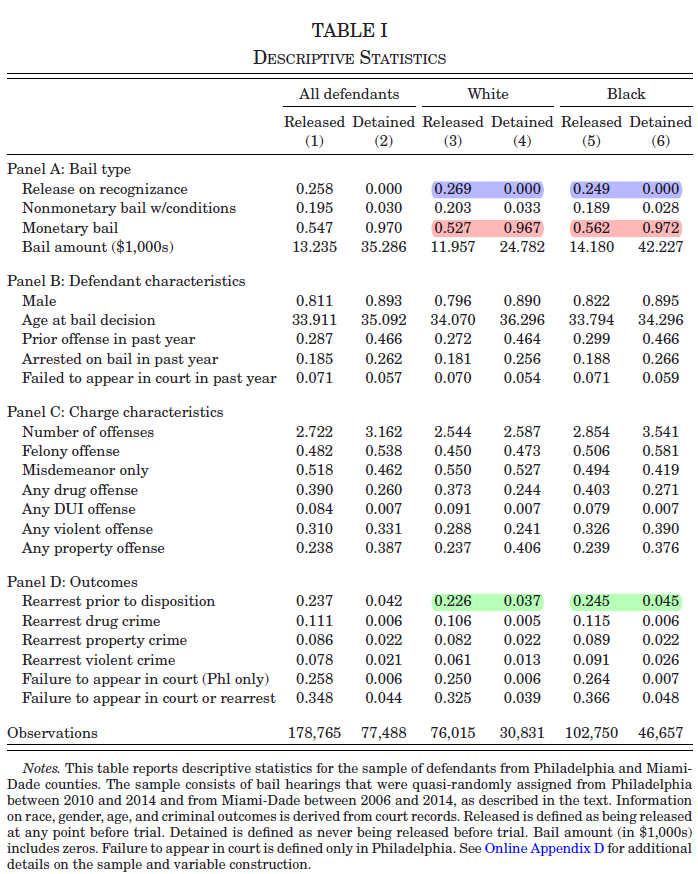
\includegraphics[scale = 1]{os0707tanji/ADY_T1}
    \end{figure}

    \begin{itemize}
      \item Black defendants are 2.4 percentage point more likely to be detained pretrial.
    \end{itemize}

    \paragraph{Construction of the IV}

    \begin{itemize}
      \item Instrument for release: quasi-rondom assignment of bail judge.
      \begin{itemize}
        \item A rotation system to balance caseloads.
      \end{itemize}
      \item A residualized, leave-out leniency measure. (Dobbie, Goldin, and Yang, 2018)
      \begin{itemize}
        \item Regression of pretrial release decisions on court-by-time fixed effects.
        \begin{itemize}
          \item court-by-bail, year-by-bail, day of week, (week-by-bail, shift-by-bail, only for Philadelphia).
        \end{itemize}
        \item Calcurate the leave-out mean judge release rate for each defenant, using the residuals.
      \end{itemize}
    \end{itemize}

    \begin{figure}[h]
      \centering
      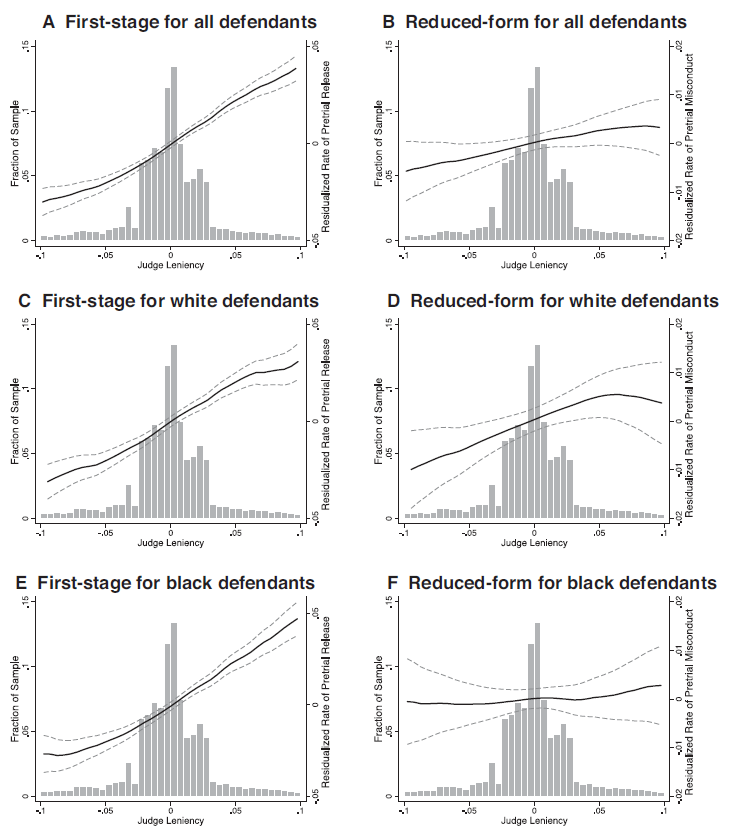
\includegraphics[scale = 1]{os0707tanji/ADY_F1}
    \end{figure}

    \begin{itemize}
      \item The judge release measure ranges in $[-.283, .253]$: moving from the least to most lenient judge increases the probability of pretrial release by 53.6 percentage points.
    \end{itemize}

    \paragraph{Instrument Validity}
    \begin{enumerate}
      \item Existance of the first stage
      \begin{itemize}
        \item They regress whether a defendant is release on the judge leniency and court-by-time fixed effects by lenear-probability model.
        \begin{align*}
          \text{Released}_{itj} &= \gamma_w Z_{itj} + \pi_W \mathbf{X}_{it} + v_{itj}, \\
          \text{Released}_{itj} &= \gamma_B Z_{itj} + \pi_B \mathbf{X}_{it} + v_{itj}
        \end{align*}
        \item $i$: defendant-case, $j$: judge, $t$: time
        \item Robust standard erros are clustered at the individual and judge-by-shift level.
        \begin{figure}[h]
          \centering
          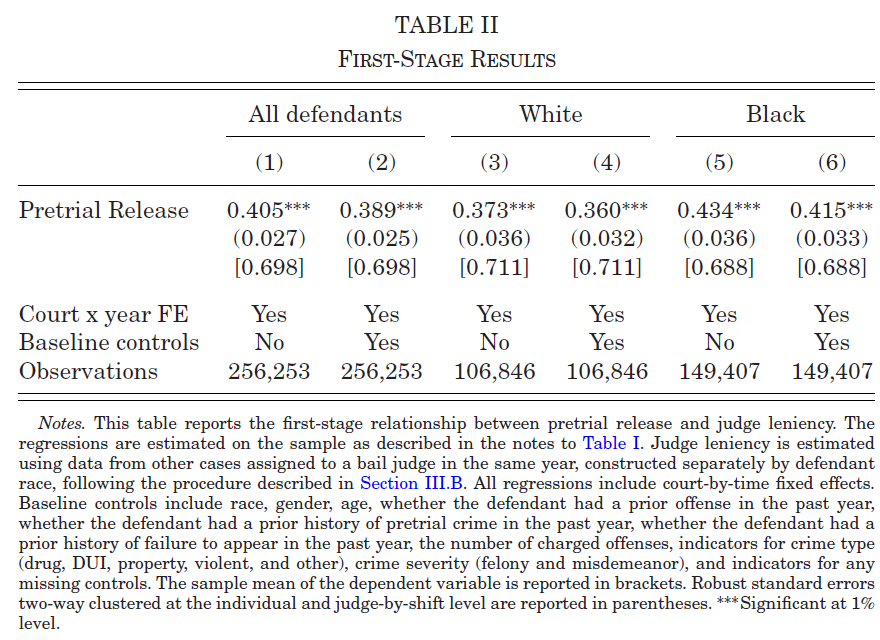
\includegraphics[scale = .8]{os0707tanji/ADY_T2}
        \end{figure}
        \item Instrumental Validity
        \begin{enumerate}
          \item Local linear regression
          \item First-stage regression
        \end{enumerate}
        \begin{itemize}
          \item The residualized judge instrument is highly predictive of whether a defendant is released pretrial.
        \end{itemize}
      \end{itemize}
      \item Exclusion Restriction
      \begin{itemize}
        \item A number of controls affect the probability of pretrial release: gender, prior offence in the past year, \dots
        \item On the other hand, judges with differeing leniencies are assigned cases with very similar defendants.
      \end{itemize}
      \begin{figure}[h]
        \centering
        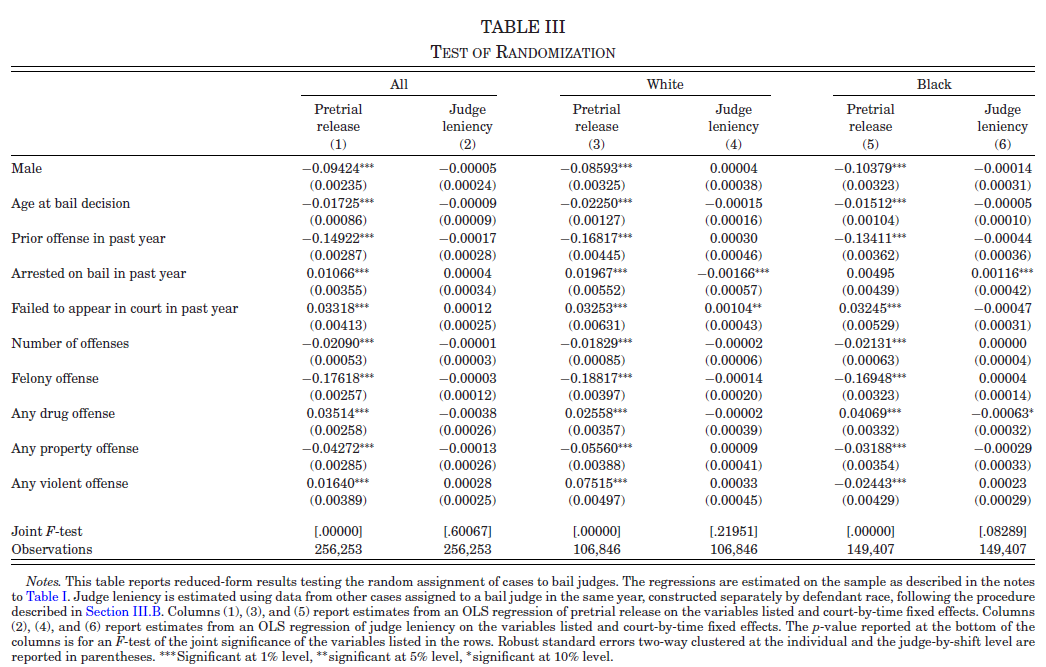
\includegraphics[scale = .8]{os0707tanji/ADY_T3}
      \end{figure}
      \begin{itemize}
        \item The exclusion restriction assumption is fundamentally untestable, but seems to be reasonable in this setting.
        \begin{itemize}
          \item Bail judges' potential channels to affect defendants is limited.
          \item There are no independent effects of the money bail amount or nonmonetary bail conditions on defendant outcomes.
          \item Bail judge assignment is uncorrelated with the assignment of public defenders and trial judges (Dobbie, Goldin, and Yang 2018)
        \end{itemize}
      \end{itemize}
      \item Monotonicity: Required to identify and interpret the IV estimator as a well-defined LATE and to estimate MTE using the standard LIV approach.
      \begin{itemize}
        \item The observed judge behavior only imperfectly monotonic with respect to race.
        \begin{itemize}
          \item A regression of the ranking of each judge's leniency for whites on that for blacks yealds a cefeecient equal to .827 (std.err. = .010).
        \end{itemize}
      \end{itemize}
    \end{enumerate}

    \section{Results}

    \subsection{Empirical Test for Racial Bias}

    \paragraph{IV Estimates}

    \begin{itemize}
      \item Two-stage least squares specifications.
      \begin{align*}
        Y_{itj} &= \alpha_W^{\text{IV}}\text{Released}_{itj} + \beta_W \mathbf{X}_{it} + \mathbf{v}_{itj} \\
        Y_{itj} &= \alpha_B^{\text{IV}}\text{Released}_{itj} + \beta_B \mathbf{X}_{it} + \mathbf{v}_{itj}
      \end{align*}
      \begin{itemize}
        \item $\mathbf{X}_{it}$: court-by-time fixed effects and baseline crime and defendant controls: race, gender, age, whether the defendant had a prior offense in the past year, whether the defendant had a prior history of pretrial crime in the past year, whether the defendant had a prior history of failure to appear in the past year, the number of charged offenses, indicators for crime type (drug, DUI, property, violent, or other), crime severity (felony or misdemeanor), and indicators for any missing characteristics.
      \end{itemize}
      \item Results: Conving evidence of racial bias against black defendants.
      \begin{itemize}
        \item Marginally released white defendants are 23.6 percentage points more likely to be rearrested for any crime, while for marginally released black defendants the effect size is a statistically insignificant 1.4 percentage points.
        \item marginally released white defendants are 22.2 percentage points more likely to be rearrested ($p = .027$)
      \end{itemize}
    \end{itemize}


    \paragraph{MTE Estimates}

    \begin{itemize}
      \item MTE estimator allows to put equal weight on each judge in the sample with additional auxiliary assumptions.
      \item Procedure
      \begin{enumerate}
        \item The entire distribution of MTEs are given as the derivative of residualized rearrest before case disposition, $\ddot{Y}_{itj}$, w.r.t. variation in the propensity score.
        \begin{align*}
          \text{MTE}_W \left(p_W^j \right) &= \dfrac{\partial}{\partial p_W^j} E(\ddot{Y}_{itj} | p_W^j, W) \\
          \text{MTE}_B \left(p_B^j \right) &= \dfrac{\partial}{\partial p_B^j} E(\ddot{Y}_{itj} | p_B^j, B)
        \end{align*}
        \begin{itemize}
          \item $\ddot{Y}_{itj}$: rearrest residualized using the full set of court-by time FEs and controls $\mathbf{X}_{it}$.
          \item $p_r^i$: the propensity score calculated by the regression of the resudualized release variable on the rezidualized judge leniency (cf. Heckman, Urzua, adn Vytlacil, 2006; Doyle, 2007).
        \end{itemize}
        \item Calculate the level of racial bias for each judge $j$.
        \begin{itemize}
          \item The average of bias across all bail judges using a simple average of the judge-specific estimates:
          \[
          D^{\text{MTE}} = \sum_{j = 1}^J \dfrac{1}{J} \left( \text{MTE}_W(p_W^j) - \text{MTE}_B(p_B^j) \right)
          \]
          \item Standard errors are calculated by bootstrapping.
        \end{itemize}
      \end{enumerate}
      \item Results
      \begin{itemize}
        \item marginally released white defendants are 24.9 percentage points more likely to be rearrested for any crime, while that for black defendants is a statistically insignificant 1.7 percentage points (column (5)).
        \item marginally released white defendants are 23.1 percentage points ($p = .048$) more likely to be rearrested.
        \item (Figure 2) the MTEs for white defendants lie strictly above the MTEs for black defendants: racial bias against black defendants at every part of the judge leniency distribution.
      \end{itemize}
    \end{itemize}

    \begin{figure}[h]
      \centering
      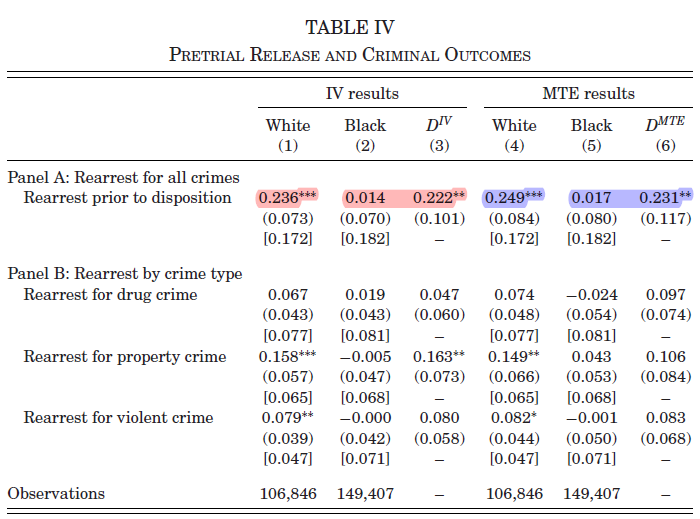
\includegraphics[scale = 1]{os0707tanji/ADY_T4}
    \end{figure}

    \begin{figure}[h]
      \centering
      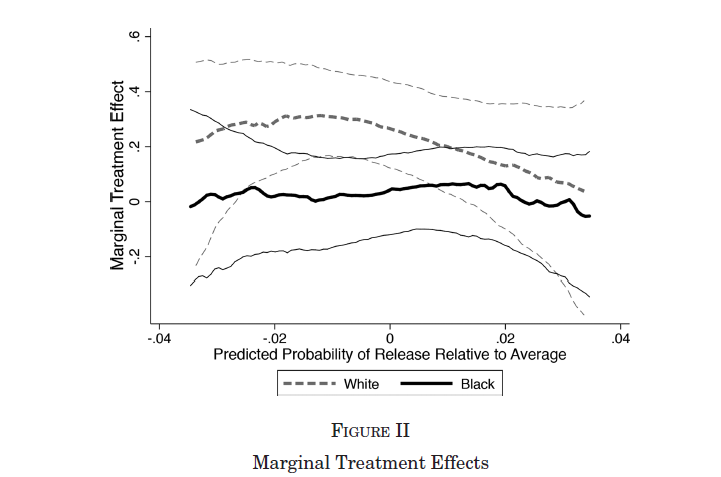
\includegraphics[scale = 1]{os0707tanji/ADY_F2}
    \end{figure}

    \paragraph{Robustness}

    \begin{itemize}
      \item They explore whether the results are subject to omitted payoff bias.
      \begin{itemize}
        \item Definition of pretrial misconducts: only failure to appear, only rearrest.
        \item Subset of more serious crimes
        \item Drop defendants who were rearrested despite never being released.
        \item Comparing outcomes for marginal non-Hispanic white and black defendants.
        \item Specification that monetary bail amounts have an independent effect on the probability of pretrial misconduct.
      \end{itemize}
      Under each alternative specifications, consistent evidence of racial bias against black defendants.
    \end{itemize}

    \paragraph{Comparison to Other Outcome Tests}

    \begin{itemize}
      \item Knowles, Perisco, and Todd (2001): standard OLS does not report that the average pretrial misconduct rate will not vary by defendant race.

      $\Rightarrow$ In this paper, standard OLS estimates suggest racial bias against \textbf{white} defendants.
      \item Anwar and Fang (2006): under the null hypothesis, the treatment of black and white defendants will not depend on judge race.

      $\Rightarrow$ Both white and black judges are racially biased against black defendants.
    \end{itemize}

    Taken together, the results highlight the importance of accounting for inframarginality and omitted variables.

    \section{Potential Mechanisms}

    \subsection{Racial Animus}

    \begin{itemize}
      \item Judges may either knowingly or unknowingly discriminate against black defendants at the margin of release (Becker; 1957, 1993)
      \begin{itemize}
        \item[ex.)] Judges coule harbor explicit animus against black defendants that leads them to value the freedom of black defendants less than that of whites.
        \item Racial prejudice is most likely to translate into the disparate treatment of minorities.
      \end{itemize}
      \item Suggestive piece of evidence against this is provided by Anwar and Fang (2006) test of relative racial bias.
      \begin{itemize}
        \item IV and MTE estimates of racial bias are similar among white and black judges:

        $\Rightarrow$ either racial animus is not driving our results or that black and white bail judges harbor equal levels of racial animus toward black defendants.
      \end{itemize}
    \end{itemize}

    \subsection{Racially Biased Prediction}

    \begin{itemize}
      \item Bail Judges are making racially biased prediction errors in risk.
      \begin{itemize}
        \item Bordalo et al. (2016): Representative heuristics can exaggerate perceived differences between groups.
      \end{itemize}
      \item The race-based prediction errors exacerbated by the fact that judges must make quick judgments on the basis of limited information and with virtually no training.
    \end{itemize}

    \paragraph{Representativeness of Black and White Defendants}

    \begin{itemize}
      \item The antiblack stereotypes are present $\Leftrightarrow$ blacks are overrepresented among the right tail of the predicted risk distribution relative to whites: Judges believe that black defendants are riskier than they actually are.
      \item (Figure 3) Black defendants are significantly underrepresented in the left tail and overrepresented in the right tail of the predicted risk distribution: Black defendants are
      \begin{itemize}
        \item 1.2 times less likely than whites to be represented among the bottom 25\% of the predicted risk distribution.
        \item 1.1 more among the top 25\%.
      \end{itemize}
      \item If judges apply the same release threshold for whites to blacks,  70.8\% of black defendants are to be released, while in practice only 68.8\% are released pretrial.
    \end{itemize}

    \begin{figure}[h]
      \centering
      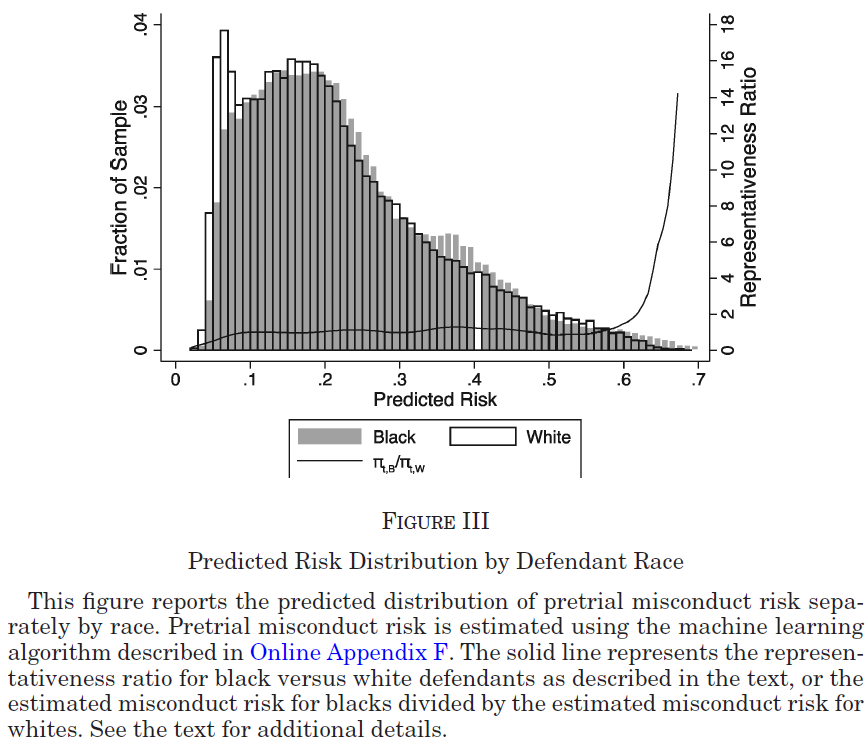
\includegraphics[scale = .7]{os0707tanji/ADY_F3}
    \end{figure}

    \newpage

    \subparagraph{Sterotype Model}: Representativeness-based discounting model

    \begin{itemize}
      \item The stereotyped beliefs for black defendants, $\pi_{t, B}^{\text{st}}$
      \[
      \pi_{t, B}^{\text{st}} = \pi_{t, B}
      \dfrac{\left( \dfrac{\pi_{t, B}}{\pi_{t, W}} \right)^\theta}
      {\sum_{s \in T} \pi_{t, B} \left( \dfrac{\pi_{s, B}}{\pi_{s, W}} \right)^\theta}
      \]
      \begin{itemize}
        \item $r, t$ denotes the defendant's race and the risk type, respectively.
        \item $\theta$: the extent to which representativeness distorts beliefs and the representativeness ratio.
      \end{itemize}
      \item Setting $\theta = 1.9$, the true average release rate for blacks is rationalized: The mean predicted risk is .235 under true distribution, compared with .288 under stereotyped distribution.
      \item Crime-specific distributions, and comparison of the Hispanic and black to the non-Hispanic white do not change the interpretation.
      \begin{figure}[h]
        \centering
        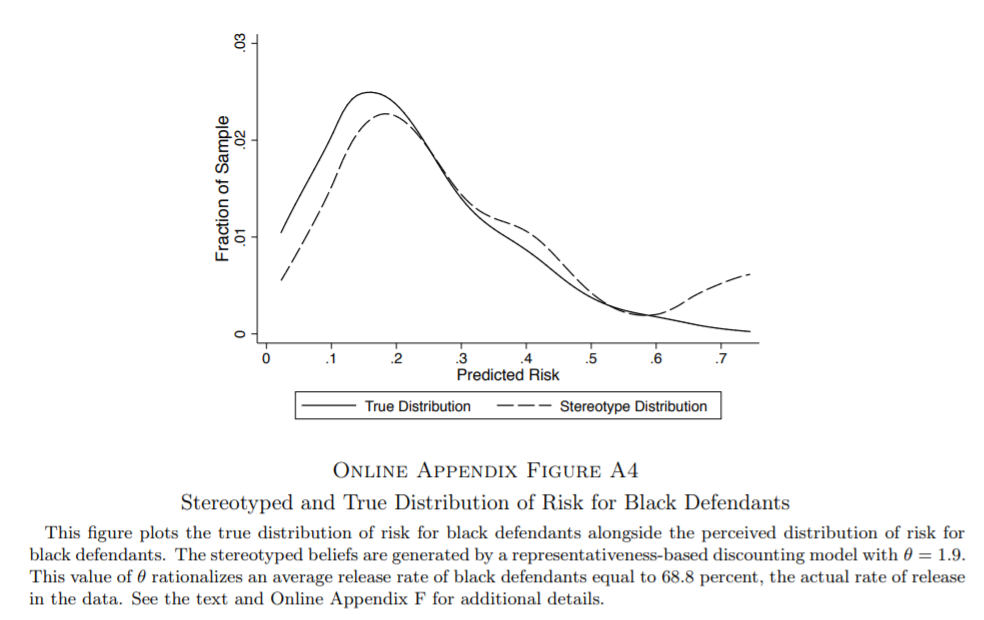
\includegraphics[scale = 1]{os0707tanji/ADY_FA4}
      \end{figure}
    \end{itemize}

    \paragraph{Racial Bias and Prediction Errors in Risk}

    \begin{itemize}
      \item Where prediction errors are more likely to occur?
      \item One such test: A comparison of experienced and inexperienced judges.
      \begin{itemize}
        \item Consistent with this idea, more experienced judges are more likely to release defendants, but not make misclassification errors.
      \end{itemize}
      \item Differences by city: Bail judges in Philadelphia specialize in setting bail, while in Miami, they are part-time generalists.
      \begin{itemize}
        \item Racial bias is higher in Miami than Philadelphia, although the difference is insignificant.
      \end{itemize}
      \item Additional evidence: Variation in the experience in Miami.
    \end{itemize}

    \begin{figure}[h]
      \centering
      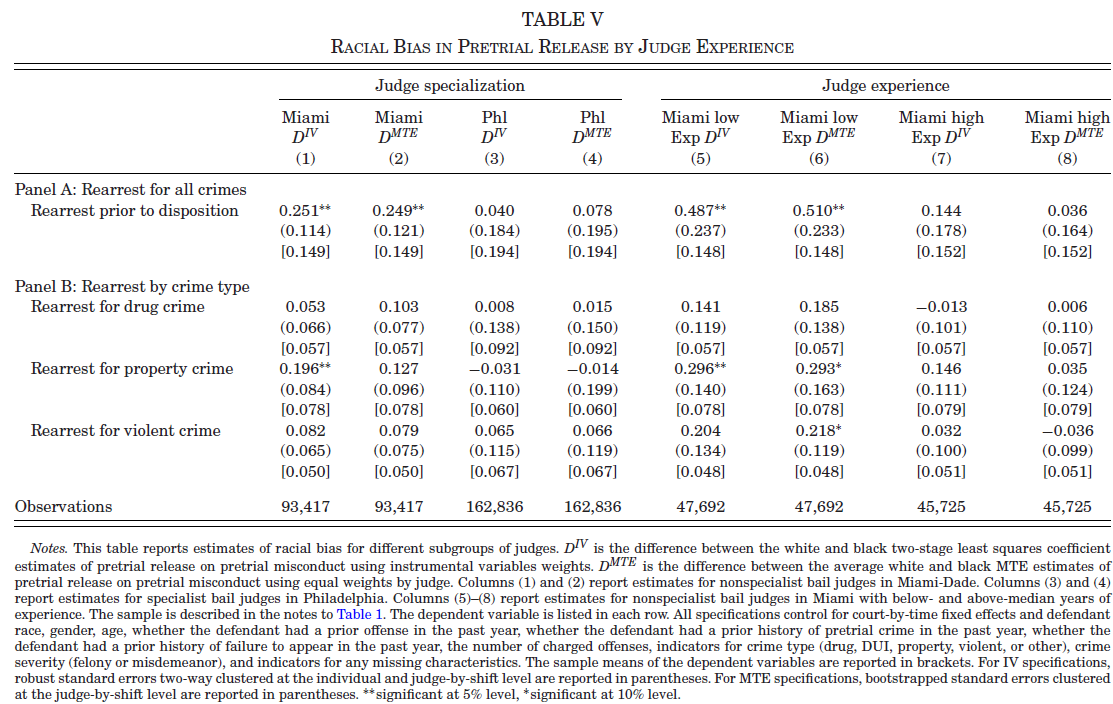
\includegraphics[scale = .7]{os0707tanji/ADY_T5}
    \end{figure}

    \newpage


    \section{Concluding Remarks}

    \paragraph{Implication}

    \begin{itemize}
      \item Racially biased prediction errors among inexperienced judges are an important driver of black

      $\Rightarrow$ providing judges with increased opportunities for training or on-the-job feedback could play an important role in decreasing racial disparities in the criminal justice system.

      \item The empirical test developed in this article can be used to test for bias in other settings.
      \begin{itemize}
        \item Quasi-random assignment of decision makers and the objective of these decision makers is both known and well measured.
      \end{itemize}
    \end{itemize}


    \biblio

\end{document}
